\documentclass[tikz,border=2pt]{standalone}
\usepackage{amsmath,amssymb}
\usepackage{pgfplots}
\pgfplotsset{compat=1.18}
\usetikzlibrary{arrows.meta}
\begin{document}
% X = 1 surely versus Y in {0,2} with probability 1/2 each: equal means, and the stop-loss transforms
% E[(X-d)_+] = (1-d)_+ <= E[(Y-d)_+] = (2-d)_+/2 for every d >= 0, so X <=_cx Y.
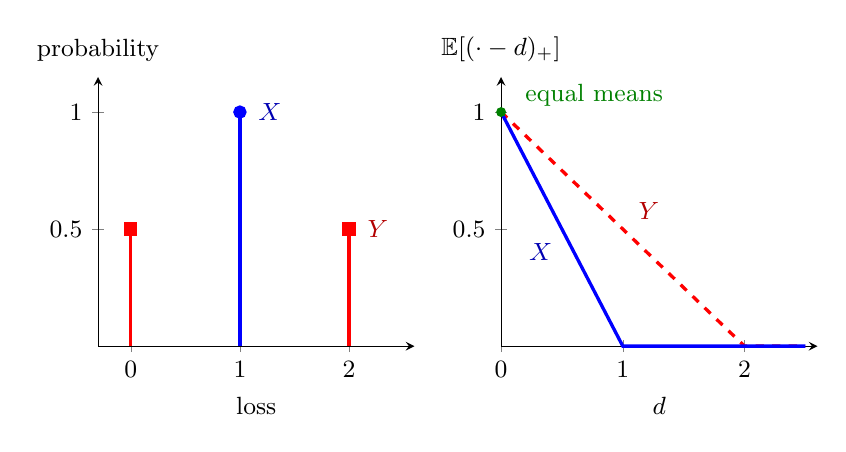
\begin{tikzpicture}[font=\small, >={Latex[length=2mm]}]
  \begin{axis}[name=left,
    axis lines=left, xmin=-0.3, xmax=2.6, ymin=0, ymax=1.15,
    xtick={0,1,2}, ytick={0.5,1},
    xlabel={loss}, ylabel={probability},
    ylabel style={rotate=-90, anchor=south, at={(axis description cs:0,1.02)}},
    width=5.6cm, height=5cm, clip=false]
    \addplot[blue, very thick, ycomb, mark=*, mark size=1.8pt, mark options={fill=blue}] coordinates {(1,1)};
    \addplot[red, very thick, ycomb, mark=square*, mark size=1.8pt, mark options={fill=red}] coordinates {(0,0.5) (2,0.5)};
    \node[blue!70!black, anchor=west] at (axis cs:1.08,1) {$X$};
    \node[red!70!black, anchor=west] at (axis cs:2.08,0.5) {$Y$};
  \end{axis}
  \begin{axis}[at={(left.east)}, anchor=west, xshift=1.1cm,
    axis lines=left, xmin=0, xmax=2.6, ymin=0, ymax=1.15,
    xtick={0,1,2}, ytick={0.5,1},
    xlabel={$d$}, ylabel={$\mathbb E[(\cdot-d)_+]$},
    ylabel style={rotate=-90, anchor=south, at={(axis description cs:0,1.02)}},
    width=5.6cm, height=5cm, clip=false]
    \addplot[red, very thick, dashed] coordinates {(0,1) (2,0) (2.5,0)};
    \addplot[blue, very thick] coordinates {(0,1) (1,0) (2.5,0)};
    \node[red!70!black, anchor=south west] at (axis cs:1.05,0.5) {$Y$};
    \node[blue!70!black, anchor=north east] at (axis cs:0.5,0.48) {$X$};
    \fill[green!50!black] (axis cs:0,1) circle (1.8pt);
    \node[green!50!black, anchor=west] at (axis cs:0.12,1.07) {equal means};
  \end{axis}
\end{tikzpicture}
\end{document}
